\begin{center}
    \textbf{Assessment 1}
\end{center}

\begin{prob} %Problem 1 
    A driver wants to go from the one side of the city to the other, avoiding the city center. In the figure below you can see all the road-system and the numbers over the arcs represent the time needed to go from a node to the other.
    
    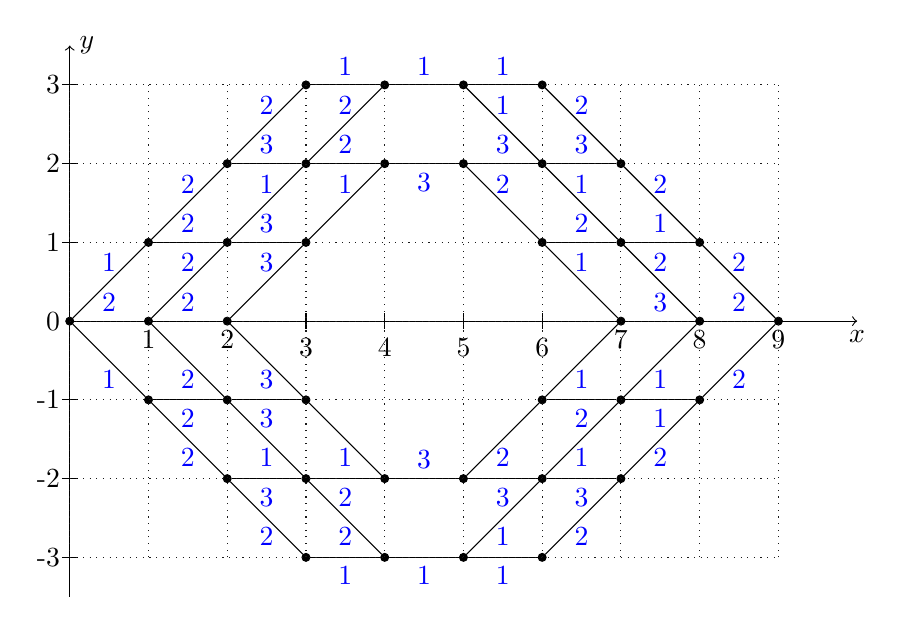
\begin{tikzpicture}
\draw[->] (0,-3.5) -- (0,3.5) node [right] {$y$};  
\draw[->] (0,0) -- (10,0) node [below] {$x$}; 

\foreach \i in {3,4,5,6}
    \draw ({\i}, 0.1) -- ({\i},-0.1) node [below] {\i};

\foreach \i in {1,2,3,-1,-2,-3}
    \draw (-0.1, {\i}) -- (0.1, {\i});
    

    
\node[circle,draw,inner sep=1pt,fill] (A00)  at (0,0) {};
\node[circle,draw,inner sep=1pt,fill] (A10)  at (1,0) {};
\node[circle,draw,inner sep=1pt,fill] (A11)  at (1,1) {};
\node[circle,draw,inner sep=1pt,fill] (A11m) at (1,-1) {};
\node[circle,draw,inner sep=1pt,fill] (A20)  at (2,0) {};
\node[circle,draw,inner sep=1pt,fill] (A21)  at (2,1)  {};
\node[circle,draw,inner sep=1pt,fill] (A22)  at (2,2) {};
\node[circle,draw,inner sep=1pt,fill] (A21m) at (2,-1)  {};
\node[circle,draw,inner sep=1pt,fill] (A22m) at (2,-2) {};
\node[circle,draw,inner sep=1pt,fill] (A31)  at (3,1)  {};
\node[circle,draw,inner sep=1pt,fill] (A32)  at (3,2) {};
\node[circle,draw,inner sep=1pt,fill] (A33)  at (3,3) {};
\node[circle,draw,inner sep=1pt,fill] (A31m) at (3,-1)  {};
\node[circle,draw,inner sep=1pt,fill] (A32m) at (3,-2) {};
\node[circle,draw,inner sep=1pt,fill] (A33m) at (3,-3) {};
\node[circle,draw,inner sep=1pt,fill] (A42)  at (4,2) {};
\node[circle,draw,inner sep=1pt,fill] (A43)  at (4,3) {};
\node[circle,draw,inner sep=1pt,fill] (A42m) at (4,-2) {};
\node[circle,draw,inner sep=1pt,fill] (A43m) at (4,-3) {};
\node[circle,draw,inner sep=1pt,fill] (A52)  at (5,2) {};
\node[circle,draw,inner sep=1pt,fill] (A53)  at (5,3) {};
\node[circle,draw,inner sep=1pt,fill] (A52m) at (5,-2) {};
\node[circle,draw,inner sep=1pt,fill] (A53m) at (5,-3) {};
\node[circle,draw,inner sep=1pt,fill] (A61)  at (6,1)  {};
\node[circle,draw,inner sep=1pt,fill] (A62)  at (6,2) {};
\node[circle,draw,inner sep=1pt,fill] (A63)  at (6,3) {};
\node[circle,draw,inner sep=1pt,fill] (A61m) at (6,-1)  {};
\node[circle,draw,inner sep=1pt,fill] (A62m) at (6,-2) {};
\node[circle,draw,inner sep=1pt,fill] (A63m) at (6,-3) {};
\node[circle,draw,inner sep=1pt,fill] (A70)  at (7,0) {};
\node[circle,draw,inner sep=1pt,fill] (A71)  at (7,1)  {};
\node[circle,draw,inner sep=1pt,fill] (A72)  at (7,2) {};
\node[circle,draw,inner sep=1pt,fill] (A71m) at (7,-1)  {};
\node[circle,draw,inner sep=1pt,fill] (A72m) at (7,-2) {};
\node[circle,draw,inner sep=1pt,fill] (A80)  at (8,0) {};
\node[circle,draw,inner sep=1pt,fill] (A81)  at (8,1) {};
\node[circle,draw,inner sep=1pt,fill] (A81m) at (8,-1) {};
\node[circle,draw,inner sep=1pt,fill] (A90)  at (9,0) {};

\node at (A00)  [left] {0};
\node at (A10)  [below] {1};
\node at (A20)  [below] {2};
\node at (A70)  [below] {7};
\node at (A80)  [below] {8};
\node at (A90)  [below] {9};

\node at (0,1) [left] {1};
\node at (0,2) [left] {2};
\node at (0,3) [left] {3};
\node at (0,-1) [left] {-1};
\node at (0,-2) [left] {-2};
\node at (0,-3) [left] {-3};


\draw (A00) -- (A10) node[blue, above, midway] {2};
\draw (A10) -- (A20) node[blue, above, midway] {2};

\draw (A00) -- (A11) node[blue, above, midway] {1};
\draw (A10) -- (A21) node[blue, above, midway] {2};
\draw (A11) -- (A21) node[blue, above, midway] {2};
\draw (A11) -- (A22) node[blue, above, midway] {2};
\draw (A20) -- (A31) node[blue, above, midway] {3};
\draw (A21) -- (A31) node[blue, above, midway] {3};
\draw (A21) -- (A32) node[blue, above, midway] {1};
\draw (A22) -- (A33) node[blue, above, midway] {2};
\draw (A32) -- (A43) node[blue, above, midway] {2};
\draw (A53) -- (A62) node[blue, above, midway] {1};
\draw (A63) -- (A72) node[blue, above, midway] {2};

\draw (A22) -- (A32) node[blue, above, midway] {3};
\draw (A32) -- (A42) node[blue, above, midway] {2};
\draw (A42) -- (A52) node[blue, below, midway] {3};
\draw (A52) -- (A62) node[blue, above, midway] {3};
\draw (A62) -- (A72) node[blue, above, midway] {3};

\draw (A31) -- (A42) node[blue, above, midway] {1};
\draw (A33) -- (A43) node[blue, above, midway] {1};
\draw (A43) -- (A53) node[blue, above, midway] {1};
\draw (A53) -- (A63) node[blue, above, midway] {1};

\draw (A52) -- (A61) node[blue, above, midway] {2};
\draw (A62) -- (A71) node[blue, above, midway] {1};
\draw (A72) -- (A81) node[blue, above, midway] {2};
\draw (A61) -- (A70) node[blue, above, midway] {1};
\draw (A71) -- (A80) node[blue, above, midway] {2};
\draw (A81) -- (A90) node[blue, above, midway] {2};

\draw (A61) -- (A71) node[blue, above, midway] {2};
\draw (A71) -- (A81) node[blue, above, midway] {1};

\draw (A70) -- (A80) node[blue, above, midway] {3};
\draw (A80) -- (A90) node[blue, above, midway] {2};



\draw (A00) -- (A11m) node[blue, below, midway] {1};
\draw (A10) -- (A21m) node[blue, below, midway] {2};
\draw (A11m) -- (A21m) node[blue, below, midway] {2};
\draw (A11m) -- (A22m) node[blue, below, midway] {2};
\draw (A20) -- (A31m) node[blue, below, midway] {3};
\draw (A21m) -- (A31m) node[blue, below, midway] {3};
\draw (A21m) -- (A32m) node[blue, below, midway] {1};
\draw (A22m) -- (A33m) node[blue, below, midway] {2};
\draw (A32m) -- (A43m) node[blue, below, midway] {2};
\draw (A53m) -- (A62m) node[blue, below, midway] {1};
\draw (A63m) -- (A72m) node[blue, below, midway] {2};

\draw (A22m) -- (A32m) node[blue, below, midway] {3};
\draw (A32m) -- (A42m) node[blue, below, midway] {2};
\draw (A42m) -- (A52m) node[blue, above, midway] {3};
\draw (A52m) -- (A62m) node[blue, below, midway] {3};
\draw (A62m) -- (A72m) node[blue, below, midway] {3};

\draw (A31m) -- (A42m) node[blue, below, midway] {1};
\draw (A33m) -- (A43m) node[blue, below, midway] {1};
\draw (A43m) -- (A53m) node[blue, below, midway] {1};
\draw (A53m) -- (A63m) node[blue, below, midway] {1};

\draw (A52m) -- (A61m) node[blue, below, midway] {2};
\draw (A62m) -- (A71m) node[blue, below, midway] {1};
\draw (A72m) -- (A81m) node[blue, below, midway] {2};
\draw (A61m) -- (A70) node[blue, below, midway] {1};
\draw (A71m) -- (A80) node[blue, below, midway] {1};
\draw (A81m) -- (A90) node[blue, below, midway] {2};

\draw (A61m) -- (A71m) node[blue, below, midway] {2};
\draw (A71m) -- (A81m) node[blue, below, midway] {1};

    \draw[black!90, dotted] (0,3) grid (9,-3);

\end{tikzpicture}
    
    \begin{enumerate}[label = {\textbf{(\greek*)}}]
        \item Find the fastest paths starting from the node $(0, 0)$, and ending at $(9, 0)$.
        
        \begin{sol}
        We use the backward method of dynamic programming
        
        The costs on the graph symmetric wrt the $x$-axis, so we need only consider the paths above the $x$-axis and then \textit{mirror} the solutions.
        
        We define the objective function $f(x,y)$ as the minimal cost from $(x,y)$ to $(9,0)$, i.e.
        
        $$f(x,y):=\min\cbr{u(x,y)+f(x+1,y+1),m(x,y)+f(x+1,y),l(x,y)+f(x+1,y-1)}$$
        
        Where \begin{itemize}
            \item $u(x,y)$ the cost of moving from the node $(x, y)$ to upper-node $(x + 1, y + 1)$.
            \item $m(x,y)$ the cost of moving from the node $(x, y)$ to middle-node $(x + 1, y)$.
            \item $l(x,y)$ the cost of moving from the node $(x, y)$ to lower-node $(x + 1, y - 1)$.
        \end{itemize}
        
        If no such node exists for one of these costs, the value is $\infty$.
        
        We have the boundary condition $f(9,0)=0$ and we wish to find $f(0,0)$
        
        We will also use decision function $d(x,y)=$ the choice of the next node, to work out the optimal path(s).

        
        \begin{itemize}
            \item[$\underline{x=9}$] Points: $(9,0)$
            
            $f(9,0)=0$ (Boundary Condition)
            
            \item[$\underline{x=8}$] Points: $(8,1), \ (8,0)$
            
            $\begin{aligned}
            f(8,1) &= \min\cbr{
            u(8,1)+f(9,2),m(8,1)+f(9,1),l(8,1)+f(9,0)}\\
            &= \min\cbr{ \infty,\infty,2+0} = 2 & d(8,1)=(9,0)\\
            f(8,0) &= \min\cbr{
            u(8,0)+f(9,1),m(8,0)+f(9,0),l(8,0)+f(9,-1)}\\
            &= \min\cbr{ \infty,2+0,\infty} = 2 & d(8,0)=(9,0)
            \end{aligned}$
            
            \item[$\underline{x=7}$] Points: $(7,2), \ (7,1), \ (7,0)$
            
            $\begin{aligned}
            f(7,2) &= \min\cbr{
            u(7,2)+f(8,3),m(7,2)+f(8,2),l(7,2)+f(8,1)}\\
            &= \min\cbr{\infty,\infty,2+2} =4  & d(7,2)=(8,1)\\
            f(7,1) &= \min\cbr{
            u(7,1)+f(8,2),m(7,1)+f(8,1),l(7,1)+f(8,0)}\\
            &= \min\cbr{\infty,1+2,1+2} =3  & d(7,1)=(8,1) \text{ or } (8,0)\\
            f(7,0) &= \min\cbr{
            u(7,0)+f(8,1),m(7,0)+f(8,0),l(7,0)+f(8,-1)}\\
            &= \min\cbr{\infty,3+2,\infty} =5  & d(7,0)=(8,0)
            \end{aligned}$
            
            \item[$\underline{x=6}$] Points: $(6,3), \ (6,2), \ (6,1)$
            
            $\begin{aligned}
            f(6,3) &= \min\cbr{
            u(6,3)+f(7,4),m(6,3)+f(7,3),l(6,3)+f(7,2)}\\
            &= \min\cbr{\infty,\infty,2+4} =6  & d(6,3)=(7,2)\\
            f(6,2) &= \min\cbr{
            u(6,2)+f(7,3),m(6,2)+f(6,2),l(6,2)+f(7,1)}\\
            &= \min\cbr{\infty,3+4,2+3} =5  & d(6,2)=(7,1)\\
            f(6,1) &= \min\cbr{
            u(6,1)+f(7,2),m(6,1)+f(7,1),l(6,1)+f(7,0)}\\
            &= \min\cbr{\infty,2+3,2+5} =5  & d(6,1)=(7,1)
            \end{aligned}$
            
            \item[$\underline{x=5}$] Points: $(5,3), \ (5,2)$
            
            $\begin{aligned}
            f(5,3) &= \min\cbr{
            u(5,3)+f(6,4),m(5,3)+f(6,3),l(5,3)+f(6,2)}\\
            &= \min\cbr{\infty,1+6,1+5} =6  & d(5,3)=(6,2)\\
            f(5,2) &= \min\cbr{
            u(5,2)+f(6,3),m(5,2)+f(6,2),l(5,2)+f(6,1)}\\
            &= \min\cbr{\infty,3+5,2+5} =6  & d(5,2)=(6,1)
            \end{aligned}$
            
            \item[$\underline{x=4}$] Points: $(4,3), \ (4,2)$
            
            $\begin{aligned}
            f(4,3) &= \min\cbr{
            u(4,3)+f(5,4),m(4,3)+f(5,3),l(4,3)+f(5,2)}\\
            &= \min\cbr{\infty,1+6,\infty} =7  & d(4,3)=(5,3)\\
            f(4,2) &= \min\cbr{
            u(4,2)+f(5,3),m(4,2)+f(5,2),l(4,2)+f(5,1)}\\
            &= \min\cbr{\infty,3+6,\infty} =9  & d(4,2)=(5,2)
            \end{aligned}$
            
            \item[$\underline{x=3}$] Points: $(3,3), \ (3,2), \ (3,1)$
            
            $\begin{aligned}
            f(3,3) &= \min\cbr{
            u(3,3)+f(4,4),m(3,3)+f(4,3),l(3,3)+f(4,2)}\\
            &= \min\cbr{\infty,1+7,\infty} =8  & d(3,3)=(4,3)\\
            f(3,2) &= \min\cbr{
            u(3,2)+f(4,3),m(3,2)+f(4,2),l(3,2)+f(4,1)}\\
            &= \min\cbr{2+7,2+9,\infty} =9  & d(3,2)=(4,3)\\
            f(3,1) &= \min\cbr{
            u(3,1)+f(4,2),m(3,1)+f(4,1),l(3,1)+f(4,0)}\\
            &= \min\cbr{1+9,\infty,\infty} =10  & d(3,1)=(4,2)
            \end{aligned}$
            
            \item[$\underline{x=2}$] Points: $(2,2), \ (2,1), \ (2,0)$
            
            $\begin{aligned}
            f(2,2) &= \min\cbr{
            u(2,2)+f(3,3),m(2,2)+f(3,2),l(2,2)+f(3,1)}\\
            &= \min\cbr{2+8,3+9,\infty} =10  & d(2,2)=(3,3)\\
            f(2,1) &= \min\cbr{
            u(2,1)+f(3,2),m(2,1)+f(3,1),l(2,1)+f(3,0)}\\
            &= \min\cbr{1+9,3+10,\infty} =10  & d(2,1)=(3,2)\\
            f(2,0) &= \min\cbr{
            u(2,0)+f(3,1),m(2,0)+f(3,0),l(2,0)+f(3,-1)}\\
            &= \min\cbr{3+10,\infty,\infty} =13  & d(2,0)=(3,1)
            \end{aligned}$
            
            \item[$\underline{x=1}$] Points: $(1,1), \ (1,0)$
            
            $\begin{aligned}
            f(1,1) &= \min\cbr{
            u(1,1)+f(2,2),m(1,1)+f(2,1),l(1,1)+f(2,0)}\\
            &= \min\cbr{2+10,2+10,\infty} =12  & d(1,1)=(2,2) \text{ or } (2,1)\\
            f(1,0) &= \min\cbr{
            u(1,0)+f(2,1),m(1,0)+f(2,0),l(1,0)+f(2,-1)}\\
            &= \min\cbr{2+10,2+13,\infty} =12  & d(1,0)=(2,1)
            \end{aligned}$
            
            \item[$\underline{x=0}$] Final point: $(0,0)$
            
            $\begin{aligned}
            f(0,0) &= \min\cbr{
            u(0,0)+f(1,1),m(0,0)+f(1,0)} & \text{ignoring } l(0,0) \\
            &= \min\cbr{1+12,2+12,\infty} =\underbrace{13}_{\mathclap{\text{Total cost}}}  & d(0,0)=(1,1)
            \end{aligned}$
            
            Decision for the routes:
            
            $(0,0)\to(1,1)\to(2,1)\to(3,2)\to(4,3)\to(5,3)\to(6,2)\to(7,1)\to(8,1)\to(9,0)$ 
            
            $(0,0)\to(1,1)\to(2,2)\to(3,3)\to(4,3)\to(5,3)\to(6,2)\to(7,1)\to(8,1)\to(9,0)$ 
            
            $(0,0)\to(1,1)\to(2,1)\to(3,2)\to(4,3)\to(5,3)\to(6,2)\to(7,1)\to(8,0)\to(9,0)$
            
            $(0,0)\to(1,1)\to(2,2)\to(3,3)\to(4,3)\to(5,3)\to(6,2)\to(7,1)\to(8,0)\to(9,0)$
            
            We also can reflect along the $x$-axis to get
            
            $(0,0)\to(1,\text{-}1)\to(2,\text{-}1)\to(3,\text{-}2)\to(4,\text{-}3)\to(5,\text{-}3)\to(6,\text{-}2)\to(7,\text{-}1)\to(8,\text{-}1)\to(9,0)$
            
            $(0,0)\to(1,\text{-}1)\to(2,\text{-}2)\to(3,\text{-}3)\to(4,\text{-}3)\to(5,\text{-}3)\to(6,\text{-}2)\to(7,\text{-}1)\to(8,\text{-}1)\to(9,0)$
            
            $(0,0)\to(1,\text{-}1)\to(2,\text{-}1)\to(3,\text{-}2)\to(4,\text{-}3)\to(5,\text{-}3)\to(6,\text{-}2)\to(7,\text{-}1)\to(8,0)\to(9,0)$
            
            $(0,0)\to(1,\text{-}1)\to(2,\text{-}2)\to(3,\text{-}3)\to(4,\text{-}3)\to(5,\text{-}3)\to(6,\text{-}2)\to(7,\text{-}1)\to(8,0)\to(9,0)$
            
            To get 8 paths, each with total cost $13$.
        \end{itemize}
        \end{sol}
        
        \item A new path from the node $(4, 2)$ to $(5, 3)$ will open and the time needed to pass from this is $t > 0$. Find the set of the values of $t$ such that: the new optimal paths to include the motion from $(4, 2)$ to $(5, 3)$ and be faster than what you found in $\mathbf{(\alpha)}$.
        
        \begin{sol}
        We want the new path to be the choice which changes the decision at $f(4,2)$, i.e.
        
        $f(4,2)= \min\cbr{ u(4,2)+f(5,3),m(4,2)+f(5,2),l(4,2)+f(5,1)}$
        
        $= \min\cbr{t+6,3+6,\infty}$
        
        This implies that $t<3$ and the new $f(4,2)=6+t$,hence $d(4,2)=(5,3)$
        
        We can also look at 
        
        $f(3,2)= \min\cbr{ u(3,2)+f(4,3),m(3,2)+f(4,2),l(3,2)+f(4,1)}$
        
        $=\min\cbr{\infty,8+t,2+7}$ which implies that $t<1$
        
        We already require $t>0$ and so $0<t<1$
        
        Our total cost would then be strictly between $12$ and $13$, which is better than the routes from $\mathbf{(\alpha)}.$
        \end{sol}

    \end{enumerate}
\end{prob}

\pagebreak
\begin{prob} %Problem 2 
    A mathematician starts from Tralee at 6:30am and he drives to Dublin, where he is supposed to teach at 11am. Given that in several highways there are taking place constructions, the necessary time in minutes to go from the several cities to the others are given below:
    
    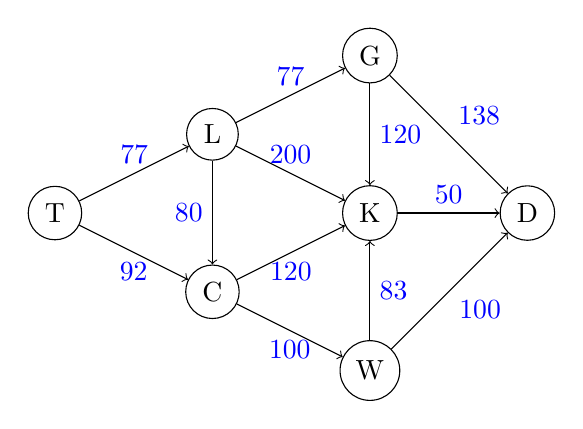
\begin{tikzpicture}
\node[circle,draw, fill = white] (T)  at (0,0) {T};
\node[circle,draw, fill = white] (L)  at (2,1) {L};
\node[circle,draw, fill = white] (C)  at (2,-1) {C};
\node[circle,draw, fill = white] (G)  at (4,2) {G};
\node[circle,draw, fill = white] (K)  at (4,0) {K};
\node[circle,draw, fill = white] (W)  at (4,-2) {W};
\node[circle,draw, fill = white] (D)  at (6,0) {D};

\draw[->] (T) -- (L) node[blue, above, midway] {77};
\draw[->] (T) -- (C) node[blue, below, midway] {92};
\draw[->] (L) -- (C) node[blue, left, midway] {80};
\draw[->] (L) -- (G) node[blue, above, midway] {77};
\draw[->] (L) -- (K) node[blue, above, midway] {200};
\draw[->] (C) -- (K) node[blue, below, midway] {120};
\draw[->] (C) -- (W) node[blue, below, midway] {100};
\draw[->] (G) -- (K) node[blue, right, midway] {120};
\draw[->] (W) -- (K) node[blue, right, midway] {83};
\draw[->] (G) -- (D) node[blue, above right, midway] {138};
\draw[->] (K) -- (D) node[blue, above, midway] {50};
\draw[->] (W) -- (D) node[blue, below right, midway] {100};

\end{tikzpicture}
    
    \begin{enumerate}[label = {\textbf{(\greek*)}}]
        \item Help him catch his class by finding the fastest path starting from Tralee to Dublin.
        
        \begin{sol}
        
        We have cities $T(0,0)$, $L(1,1)$, $C(1,-1)$, $G(2,2)$, $K(2,0)$, $W(2,-2)$ and $D(3,0)$.
        
        We use the forward method of dynamic programming.
        
        This is a \textit{general network} without circles, and so we can derive a numbering $\cbr{1,\dots,7}$ such that the costs $\alpha_{ji}$ implies $j<i$.
        
    \fbox{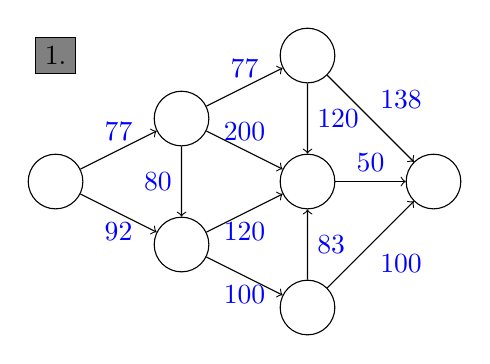
\begin{tikzpicture}[scale = 0.8]
    \node[fill = gray, shape=rectangle,draw,minimum size=8pt] (O) at (0,2)  {1.};
\node[circle,draw, fill = white, minimum size=8pt] (T)  at (0,0) {\parbox{2cm}{\par\bigskip}};
\node[circle,draw, fill = white, minimum size=8pt] (L)  at (2,1) {\parbox{2cm}{\par\bigskip}};
\node[circle,draw, fill = white, minimum size=8pt] (C)  at (2,-1) {\parbox{2cm}{\par\bigskip}};
\node[circle,draw, fill = white, minimum size=8pt] (G)  at (4,2) {\parbox{2cm}{\par\bigskip}};
\node[circle,draw, fill = white, minimum size=8pt] (K)  at (4,0) {\parbox{2cm}{\par\bigskip}};
\node[circle,draw, fill = white, minimum size=8pt] (W)  at (4,-2) {\parbox{2cm}{\par\bigskip}};
\node[circle,draw, fill = white, minimum size=8pt] (D)  at (6,0) {\parbox{2cm}{\par\bigskip}};

\draw[->] (T) -- (L) node[blue, above, midway] {77};
\draw[->] (T) -- (C) node[blue, below, midway] {92};
\draw[->] (L) -- (C) node[blue, left, midway] {80};
\draw[->] (L) -- (G) node[blue, above, midway] {77};
\draw[->] (L) -- (K) node[blue, above, midway] {200};
\draw[->] (C) -- (K) node[blue, below, midway] {120};
\draw[->] (C) -- (W) node[blue, below, midway] {100};
\draw[->] (G) -- (K) node[blue, right, midway] {120};
\draw[->] (W) -- (K) node[blue, right, midway] {83};
\draw[->] (G) -- (D) node[blue, above right, midway] {138};
\draw[->] (K) -- (D) node[blue, above, midway] {50};
\draw[->] (W) -- (D) node[blue, below right, midway] {100};
\end{tikzpicture}}
    \fbox{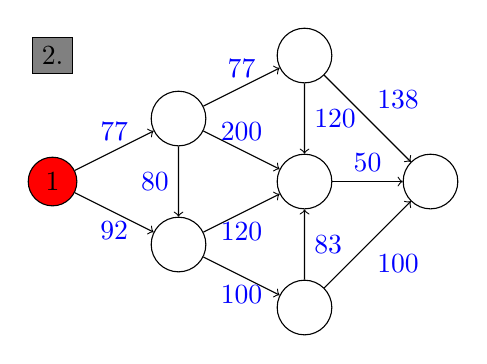
\begin{tikzpicture}[scale = 0.8]
    \node[fill = gray, shape=rectangle,draw,minimum size=8pt] (O) at (0,2)  {2.};
\node[fill = red, circle,draw, minimum size=8pt] (T)  at (0,0) {1};
\node[circle,draw, fill = white, minimum size=8pt] (L)  at (2,1) {\parbox{2cm}{\par\bigskip}};
\node[circle,draw, fill = white, minimum size=8pt] (C)  at (2,-1) {\parbox{2cm}{\par\bigskip}};
\node[circle,draw, fill = white, minimum size=8pt] (G)  at (4,2) {\parbox{2cm}{\par\bigskip}};
\node[circle,draw, fill = white, minimum size=8pt] (K)  at (4,0) {\parbox{2cm}{\par\bigskip}};
\node[circle,draw, fill = white, minimum size=8pt] (W)  at (4,-2) {\parbox{2cm}{\par\bigskip}};
\node[circle,draw, fill = white, minimum size=8pt] (D)  at (6,0) {\parbox{2cm}{\par\bigskip}};

\draw[->] (T) -- (L) node[blue, above, midway] {77};
\draw[->] (T) -- (C) node[blue, below, midway] {92};
\draw[->] (L) -- (C) node[blue, left, midway] {80};
\draw[->] (L) -- (G) node[blue, above, midway] {77};
\draw[->] (L) -- (K) node[blue, above, midway] {200};
\draw[->] (C) -- (K) node[blue, below, midway] {120};
\draw[->] (C) -- (W) node[blue, below, midway] {100};
\draw[->] (G) -- (K) node[blue, right, midway] {120};
\draw[->] (W) -- (K) node[blue, right, midway] {83};
\draw[->] (G) -- (D) node[blue, above right, midway] {138};
\draw[->] (K) -- (D) node[blue, above, midway] {50};
\draw[->] (W) -- (D) node[blue, below right, midway] {100};
\end{tikzpicture}} 
    \fbox{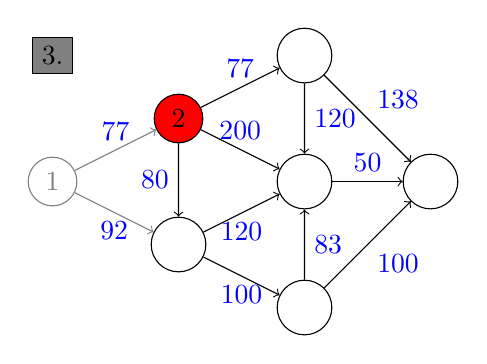
\begin{tikzpicture}[scale = 0.8]
    \node[fill = gray, shape=rectangle,draw,minimum size=8pt] (O) at (0,2)  {3.};
\node[gray, circle,draw, minimum size=8pt] (T)  at (0,0) {1};
\node[fill = red, circle,draw, minimum size=8pt] (L)  at (2,1) {2};
\node[circle,draw, fill = white, minimum size=8pt] (C)  at (2,-1) {\parbox{2cm}{\par\bigskip}};
\node[circle,draw, fill = white, minimum size=8pt] (G)  at (4,2) {\parbox{2cm}{\par\bigskip}};
\node[circle,draw, fill = white, minimum size=8pt] (K)  at (4,0) {\parbox{2cm}{\par\bigskip}};
\node[circle,draw, fill = white, minimum size=8pt] (W)  at (4,-2) {\parbox{2cm}{\par\bigskip}};
\node[circle,draw, fill = white, minimum size=8pt] (D)  at (6,0) {\parbox{2cm}{\par\bigskip}};

\draw[gray, ->] (T) -- (L) node[blue, above, midway] {77};
\draw[gray, ->] (T) -- (C) node[blue, below, midway] {92};
\draw[->] (L) -- (C) node[blue, left, midway] {80};
\draw[->] (L) -- (G) node[blue, above, midway] {77};
\draw[->] (L) -- (K) node[blue, above, midway] {200};
\draw[->] (C) -- (K) node[blue, below, midway] {120};
\draw[->] (C) -- (W) node[blue, below, midway] {100};
\draw[->] (G) -- (K) node[blue, right, midway] {120};
\draw[->] (W) -- (K) node[blue, right, midway] {83};
\draw[->] (G) -- (D) node[blue, above right, midway] {138};
\draw[->] (K) -- (D) node[blue, above, midway] {50};
\draw[->] (W) -- (D) node[blue, below right, midway] {100};
\end{tikzpicture}} 
    \fbox{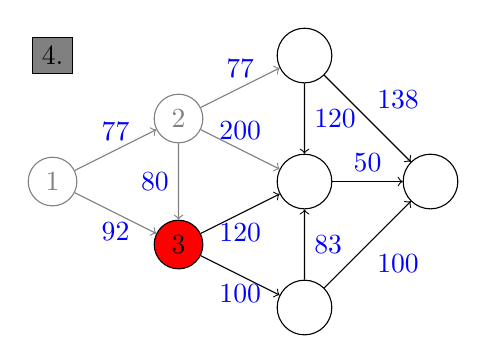
\begin{tikzpicture}[scale = 0.8]
    \node[fill = gray, shape=rectangle,draw,minimum size=8pt] (O) at (0,2)  {4.};
\node[gray, circle,draw, minimum size=8pt] (T)  at (0,0) {1};
\node[gray, circle,draw, minimum size=8pt] (L)  at (2,1) {2};
\node[fill = red, circle,draw, minimum size=8pt] (C)  at (2,-1) {3};
\node[circle,draw, fill = white, minimum size=8pt] (G)  at (4,2) {\parbox{2cm}{\par\bigskip}};
\node[circle,draw, fill = white, minimum size=8pt] (K)  at (4,0) {\parbox{2cm}{\par\bigskip}};
\node[circle,draw, fill = white, minimum size=8pt] (W)  at (4,-2) {\parbox{2cm}{\par\bigskip}};
\node[circle,draw, fill = white, minimum size=8pt] (D)  at (6,0) {\parbox{2cm}{\par\bigskip}};

\draw[gray, ->] (T) -- (L) node[blue, above, midway] {77};
\draw[gray, ->] (T) -- (C) node[blue, below, midway] {92};
\draw[gray, ->] (L) -- (C) node[blue, left, midway] {80};
\draw[gray, ->] (L) -- (G) node[blue, above, midway] {77};
\draw[gray, ->] (L) -- (K) node[blue, above, midway] {200};
\draw[->] (C) -- (K) node[blue, below, midway] {120};
\draw[->] (C) -- (W) node[blue, below, midway] {100};
\draw[->] (G) -- (K) node[blue, right, midway] {120};
\draw[->] (W) -- (K) node[blue, right, midway] {83};
\draw[->] (G) -- (D) node[blue, above right, midway] {138};
\draw[->] (K) -- (D) node[blue, above, midway] {50};
\draw[->] (W) -- (D) node[blue, below right, midway] {100};
\end{tikzpicture}} 
    \fbox{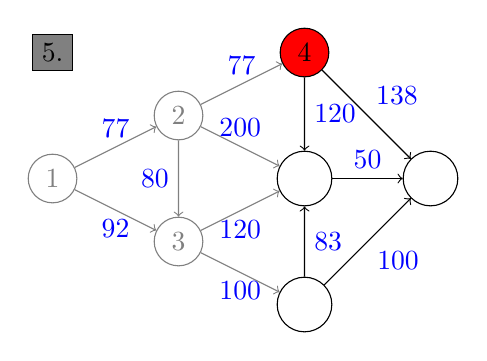
\begin{tikzpicture}[scale = 0.8]
    \node[fill = gray, shape=rectangle,draw,minimum size=8pt] (O) at (0,2)  {5.};
\node[gray, circle,draw, minimum size=8pt] (T)  at (0,0) {1};
\node[gray, circle,draw, minimum size=8pt] (L)  at (2,1) {2};
\node[gray, circle,draw, minimum size=8pt] (C)  at (2,-1) {3};
\node[fill = red, circle,draw, minimum size=8pt] (G)  at (4,2) {4};
\node[circle,draw, fill = white, minimum size=8pt] (K)  at (4,0) {\parbox{2cm}{\par\bigskip}};
\node[circle,draw, fill = white, minimum size=8pt] (W)  at (4,-2) {\parbox{2cm}{\par\bigskip}};
\node[circle,draw, fill = white, minimum size=8pt] (D)  at (6,0) {\parbox{2cm}{\par\bigskip}};

\draw[gray, ->] (T) -- (L) node[blue, above, midway] {77};
\draw[gray, ->] (T) -- (C) node[blue, below, midway] {92};
\draw[gray, ->] (L) -- (C) node[blue, left, midway] {80};
\draw[gray, ->] (L) -- (G) node[blue, above, midway] {77};
\draw[gray, ->] (L) -- (K) node[blue, above, midway] {200};
\draw[gray, ->] (C) -- (K) node[blue, below, midway] {120};
\draw[gray, ->] (C) -- (W) node[blue, below, midway] {100};
\draw[->] (G) -- (K) node[blue, right, midway] {120};
\draw[->] (W) -- (K) node[blue, right, midway] {83};
\draw[->] (G) -- (D) node[blue, above right, midway] {138};
\draw[->] (K) -- (D) node[blue, above, midway] {50};
\draw[->] (W) -- (D) node[blue, below right, midway] {100};
\end{tikzpicture}}
    \fbox{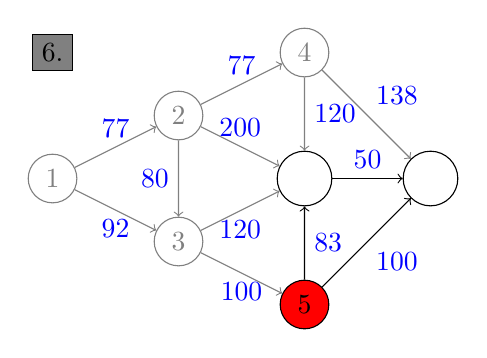
\begin{tikzpicture}[scale = 0.8]
    \node[fill = gray, shape=rectangle,draw,minimum size=8pt] (O) at (0,2)  {6.};
\node[gray, circle,draw, minimum size=8pt] (T)  at (0,0) {1};
\node[gray, circle,draw, minimum size=8pt] (L)  at (2,1) {2};
\node[gray, circle,draw, minimum size=8pt] (C)  at (2,-1) {3};
\node[gray, circle,draw, minimum size=8pt] (G)  at (4,2) {4};
\node[circle,draw, fill = white, minimum size=8pt] (K)  at (4,0) {\parbox{2cm}{\par\bigskip}};
\node[fill = red, circle,draw, minimum size=8pt] (W)  at (4,-2) {5};
\node[circle,draw, fill = white, minimum size=8pt] (D)  at (6,0) {\parbox{2cm}{\par\bigskip}};

\draw[gray, ->] (T) -- (L) node[blue, above, midway] {77};
\draw[gray, ->] (T) -- (C) node[blue, below, midway] {92};
\draw[gray, ->] (L) -- (C) node[blue, left, midway] {80};
\draw[gray, ->] (L) -- (G) node[blue, above, midway] {77};
\draw[gray, ->] (L) -- (K) node[blue, above, midway] {200};
\draw[gray, ->] (C) -- (K) node[blue, below, midway] {120};
\draw[gray, ->] (C) -- (W) node[blue, below, midway] {100};
\draw[gray, ->] (G) -- (K) node[blue, right, midway] {120};
\draw[->] (W) -- (K) node[blue, right, midway] {83};
\draw[gray, ->] (G) -- (D) node[blue, above right, midway] {138};
\draw[->] (K) -- (D) node[blue, above, midway] {50};
\draw[->] (W) -- (D) node[blue, below right, midway] {100};
\end{tikzpicture}}
    \fbox{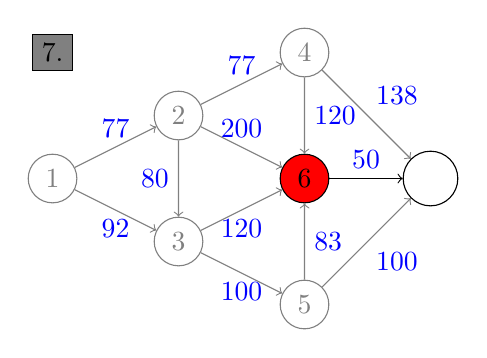
\begin{tikzpicture}[scale = 0.8]
    \node[fill = gray, shape=rectangle,draw,minimum size=8pt] (O) at (0,2)  {7.};
\node[gray, circle,draw, minimum size=8pt] (T)  at (0,0) {1};
\node[gray, circle,draw, minimum size=8pt] (L)  at (2,1) {2};
\node[gray, circle,draw, minimum size=8pt] (C)  at (2,-1) {3};
\node[gray, circle,draw, minimum size=8pt] (G)  at (4,2) {4};
\node[fill = red, circle,draw, minimum size=8pt] (K)  at (4,0) {6};
\node[gray, circle,draw, minimum size=8pt] (W)  at (4,-2) {5};
\node[circle,draw, fill = white, minimum size=8pt] (D)  at (6,0) {\parbox{2cm}{\par\bigskip}};

\draw[gray, ->] (T) -- (L) node[blue, above, midway] {77};
\draw[gray, ->] (T) -- (C) node[blue, below, midway] {92};
\draw[gray, ->] (L) -- (C) node[blue, left, midway] {80};
\draw[gray, ->] (L) -- (G) node[blue, above, midway] {77};
\draw[gray, ->] (L) -- (K) node[blue, above, midway] {200};
\draw[gray, ->] (C) -- (K) node[blue, below, midway] {120};
\draw[gray, ->] (C) -- (W) node[blue, below, midway] {100};
\draw[gray, ->] (G) -- (K) node[blue, right, midway] {120};
\draw[gray, ->] (W) -- (K) node[blue, right, midway] {83};
\draw[gray, ->] (G) -- (D) node[blue, above right, midway] {138};
\draw[->] (K) -- (D) node[blue, above, midway] {50};
\draw[gray, ->] (W) -- (D) node[blue, below right, midway] {100};
\end{tikzpicture}}
    \fbox{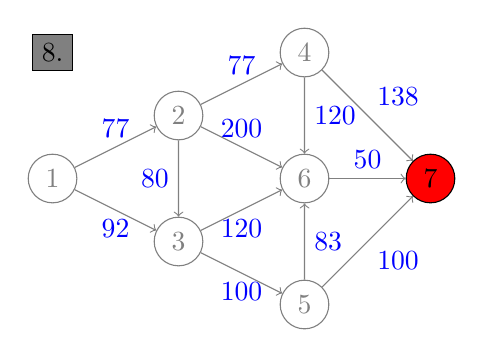
\begin{tikzpicture}[scale = 0.8]
    \node[fill = gray, shape=rectangle,draw,minimum size=8pt] (O) at (0,2)  {8.};
\node[gray, circle,draw, minimum size=8pt] (T)  at (0,0) {1};
\node[gray, circle,draw, minimum size=8pt] (L)  at (2,1) {2};
\node[gray, circle,draw, minimum size=8pt] (C)  at (2,-1) {3};
\node[gray, circle,draw, minimum size=8pt] (G)  at (4,2) {4};
\node[gray, circle,draw, minimum size=8pt] (K)  at (4,0) {6};
\node[gray, circle,draw, minimum size=8pt] (W)  at (4,-2) {5};
\node[fill = red, circle,draw, minimum size=8pt] (D)  at (6,0) {7};

\draw[gray, ->] (T) -- (L) node[blue, above, midway] {77};
\draw[gray, ->] (T) -- (C) node[blue, below, midway] {92};
\draw[gray, ->] (L) -- (C) node[blue, left, midway] {80};
\draw[gray, ->] (L) -- (G) node[blue, above, midway] {77};
\draw[gray, ->] (L) -- (K) node[blue, above, midway] {200};
\draw[gray, ->] (C) -- (K) node[blue, below, midway] {120};
\draw[gray, ->] (C) -- (W) node[blue, below, midway] {100};
\draw[gray, ->] (G) -- (K) node[blue, right, midway] {120};
\draw[gray, ->] (W) -- (K) node[blue, right, midway] {83};
\draw[gray, ->] (G) -- (D) node[blue, above right, midway] {138};
\draw[gray, ->] (K) -- (D) node[blue, above, midway] {50};
\draw[gray, ->] (W) -- (D) node[blue, below right, midway] {100};
\end{tikzpicture}}
    \fbox{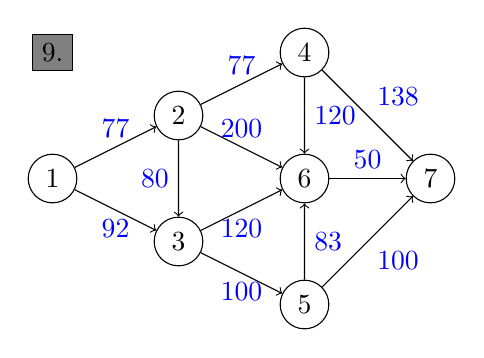
\begin{tikzpicture}[scale = 0.8]
    \node[fill = gray, shape=rectangle,draw,minimum size=8pt] (O) at (0,2)  {9.};
\node[circle,draw, minimum size=8pt] (T)  at (0,0) {1};
\node[circle,draw, minimum size=8pt] (L)  at (2,1) {2};
\node[circle,draw, minimum size=8pt] (C)  at (2,-1) {3};
\node[circle,draw, minimum size=8pt] (G)  at (4,2) {4};
\node[circle,draw, minimum size=8pt] (K)  at (4,0) {6};
\node[circle,draw, minimum size=8pt] (W)  at (4,-2) {5};
\node[circle,draw, minimum size=8pt] (D)  at (6,0) {7};

\draw[->] (T) -- (L) node[blue, above, midway] {77};
\draw[->] (T) -- (C) node[blue, below, midway] {92};
\draw[->] (L) -- (C) node[blue, left, midway] {80};
\draw[->] (L) -- (G) node[blue, above, midway] {77};
\draw[->] (L) -- (K) node[blue, above, midway] {200};
\draw[->] (C) -- (K) node[blue, below, midway] {120};
\draw[->] (C) -- (W) node[blue, below, midway] {100};
\draw[->] (G) -- (K) node[blue, right, midway] {120};
\draw[->] (W) -- (K) node[blue, right, midway] {83};
\draw[->] (G) -- (D) node[blue, above right, midway] {138};
\draw[->] (K) -- (D) node[blue, above, midway] {50};
\draw[->] (W) -- (D) node[blue, below right, midway] {100};
\end{tikzpicture}}
   
   Therefore we define the objective function
   
   $f_i:=$ the length of the shortest path from \tc{1} to \tc{$i$}.
   
   Our goal is to find $f_7$, and we also have boundary condition $f_1=0$
   
   Our recursive formula for $f_i$, by the principle of optimization (PO) is 
   
   $$f_i:= \min\limits_{j<i}\cbr{f_j+\alpha_{ji}} \quad \text{ for all } i=1,\dots,7$$
   
   Also $\alpha_{ji}:=\infty$ whenever there is no path $\tc{j}\to\tc{i}$ 
   
   $\begin{aligned}
   f_2 &= f_1 + \alpha_{12}=77 & d(2)=1\\
   f_3 &= \min\cbr{f_1+\alpha_{13},f_2+\alpha_{23}}\\
   &= \min\cbr{0+92,77+80} = 92 & d(3)=1 \\
   f_4 &= f_2 + \alpha_{24}\\
   &= 77+77 = 154 & d(4)=5 \\
   f_5 &= f_3 + \alpha_{35}\\
   &= 92+100 = 192 & d(5)=3 \\
   f_6 &= 
  \min\cbr{f_2+\alpha_{26},f_3+\alpha_{36},f_4+\alpha_{46},f_5+\alpha_{56}}\\
   &= \min\cbr{77+200,92+120,154+120,192+83} =112 & d(6)=3 \\
   f_7 &=
   \min\cbr{f_4+\alpha_{47},f_5+\alpha_{57},f_6+\alpha_{67}}\\
   &= \min\cbr{154+138,192+100,212+50} =\underbrace{262}_{\text{Total Cost}}  & d(7)=6 \\
   \end{aligned}$
   
   Therefore the fastest path is 
   
   $\tc{1}\to\tc{3}\to\tc{6}\to\tc{7}$
   
   or, for our cities,
   
   $$\trc{\text{Tralee}} \to \trc{\text{Cork}}\to\trc{\text{Kildare}}\to\trc{\text{Dublin}}$$
   
   And if he leaves at 6:30am, he will arrive at 6:30am + 262 mins $=$ 10:52am, and so he will be on time.
    \end{sol}
        
        \item Is it possible to catch his class, if the specific day, there is a quarantine in Kildare and therefore he cannot pass from this city?
        
        \begin{sol}
        We cannot include $\tc{K}$ in our route, so our new (numbered) diagram is
        
        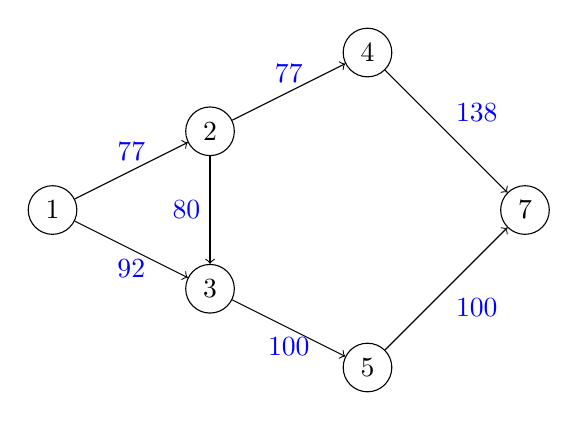
\begin{tikzpicture}
\node[circle,draw, minimum size=8pt] (T)  at (0,0)  {1};
\node[circle,draw, minimum size=8pt] (L)  at (2,1)  {2};
\node[circle,draw, minimum size=8pt] (C)  at (2,-1) {3};
\node[circle,draw, minimum size=8pt] (G)  at (4,2)  {4};
%\node[circle,draw, minimum size=8pt] (K)  at (4,0)  {K};
\node[circle,draw, minimum size=8pt] (W)  at (4,-2) {5};
\node[circle,draw, minimum size=8pt] (D)  at (6,0)  {7};

\draw[->] (T) -- (L) node[blue, above, midway] {77};
\draw[->] (T) -- (C) node[blue, below, midway] {92};
\draw[->] (L) -- (C) node[blue, left, midway] {80};
\draw[->] (L) -- (G) node[blue, above, midway] {77};
%\draw[->] (L) -- (K) node[blue, above, midway] {200};
%\draw[->] (C) -- (K) node[blue, below, midway] {120};
\draw[->] (C) -- (W) node[blue, below, midway] {100};
%\draw[->] (G) -- (K) node[blue, right, midway] {120};
%\draw[->] (W) -- (K) node[blue, right, midway] {83};
\draw[->] (G) -- (D) node[blue, above right, midway] {138};
%\draw[->] (K) -- (D) node[blue, above, midway] {50};
\draw[->] (W) -- (D) node[blue, below right, midway] {100};
\end{tikzpicture}
        
        This will only affect $f_7$ (since we no longer have an $f_6$.
        
        And so
        
        $\begin{aligned}
            f_7 &=
   \min\cbr{f_4+\alpha_{47},f_5+\alpha_{57}}\\
   &= \min\cbr{154+138,192+100} =\underbrace{292}_{\text{Total Cost}}  & d(7)=4 \text{ or } 5
        \end{aligned}$
        
        Therefore both fastest paths 
        
        $\tc{1}\to\tc{3}\to\tc{6}\to\tc{7}$ 
        \quad and \quad 
        $\tc{1}\to\tc{3}\to\tc{6}\to\tc{7}$
        
        would take $292$ minutes, but 6:30am + 292 mins $=$ 11:22am, so he will be \textbf{late}.
        \end{sol}
    \end{enumerate}
\end{prob}

\pagebreak
\begin{prob} %Problem 3 
    Using Dijkstra’s method, find the optimal route from the node \tc{1} to the node \tc{9}. The values over the arcs represent cost.
    
    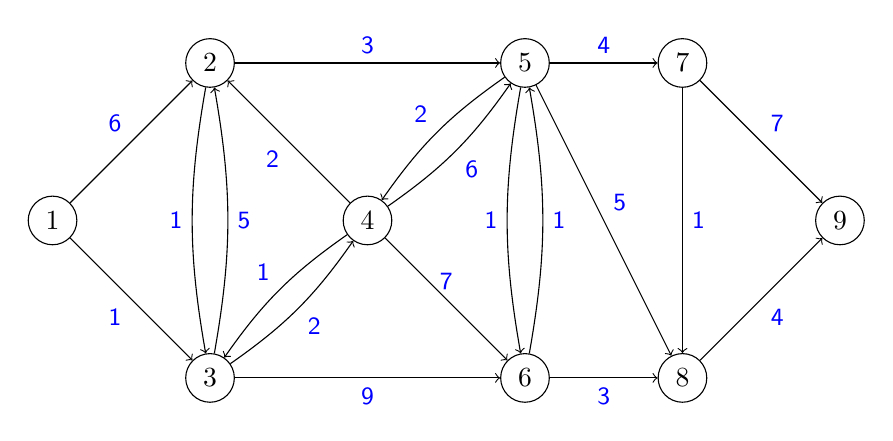
\begin{tikzpicture}
%\draw[->] (0,-2) -- (0,2) node [right] {$y$};  

%\foreach \i in {0,1,2,-1,-2}
%    \draw (-0.1, {\i}) -- (0.1, {\i}) node [left] {\i};
    
\node[circle,draw] (A1)  at (0,0) {1};
\node[circle,draw] (A2)  at (2,2) {2};
\node[circle,draw] (A3)  at (2,-2) {3};
\node[circle,draw] (A4)  at (4,0) {4};
\node[circle,draw] (A5)  at (6,2) {5};
\node[circle,draw] (A6)  at (6,-2) {6};
\node[circle,draw] (A7)  at (8,2) {7};
\node[circle,draw] (A8)  at (8,-2) {8};
\node[circle,draw] (A9)  at (10,0) {9};

\path[every node/.style={font=\sffamily\small}]
    (A1) edge[->] node [blue, pos=0.5, above left] {6} (A2)
    (A1) edge[->] node [blue, pos=0.5, below left] {1} (A3)
    (A3) edge[->, bend right=10] node [blue, pos=0.5, right] {5} (A2)
    (A2) edge[->, bend right=10] node [blue, pos=0.5, left] {1} (A3)
    (A3) edge[->, bend right=10] node [blue, pos=0.5, below right] {2} (A4)
    (A4) edge[->, bend right=10] node [blue, pos=0.5, above left] {1} (A3)
    (A4) edge[->, bend right=10] node [blue, pos=0.5, below right] {6} (A5)
    (A5) edge[->, bend right=10] node [blue, pos=0.5, above left] {2} (A4)
    (A4) edge[->] node [blue, pos=0.5, above] {7} (A6)
    (A4) edge[->] node [blue, pos=0.5, below left] {2} (A2)
    (A2) edge[->] node [blue, pos=0.5, above] {3} (A5)
    (A3) edge[->] node [blue, pos=0.5, below] {9} (A6)
    (A5) edge[->] node [blue, pos=0.5, above] {4} (A7)
    (A6) edge[->] node [blue, pos=0.5, below] {3} (A8)
    (A5) edge[bend right=10,->] node [blue, pos=0.5, left] {1} (A6)
    (A6) edge[bend right=10,->] node [blue, pos=0.5, right] {1} (A5)
    (A5) edge[->] node [blue, pos=0.5, above right] {5} (A8)
    (A7) edge[->] node [blue, pos=0.5, right] {1} (A8)
    (A7) edge[->] node [blue, pos=0.5, above right] {7} (A9)
    (A8) edge[->] node [blue, pos=0.5, below right] {4} (A9);
\end{tikzpicture}

    \begin{sol}
        We define $N_i(1):=$ the set of $i$ nodes that are closest to $\tc{1}$. Our goal is to find the minimum $i$ such that $\tc{9}\in N_i(1)$.
        
        We also define $f_i(j):=$ length of the shortest path from $\tc{1}$ to $\tc{j}$ over all nodes prior to $\tc{j}$ that belong to $N_i(1)$
        
        And $k_i$ is the $i^{\text{th}}$ closest node to $\tc{1}$, so $k_i\notin N_{i-1}(1)$.
        
        $f_{i-1}(k_i)=\min\limits_{j\notin N_{i-1}(1)}\rbr{f_{i-1}(j)}$
        
        Our recursive formula is then
        
        $$f_i(j)=\begin{cases} 
        f_{i-1}(j), & j\in N_{i}(1) \\
        \min\cbr{f_{i-1}(j),f_{i-1}(k_i)+\alpha_{k_i j}}, & j\notin N_{i}(1)
        \end{cases}$$
        
        where $\alpha_{k_i j}$ is the cost of going from node \tc{$k_i$} to node $\tc{j}$ (it is $\infty$ if there is no such path).
        
        \begin{enumerate}[label = {$\underline{i =\arabic*:}$}]
    \item 
    
    $N_1(1)=\{1\}, \ k_1=1$ (always)
    
    $f_1(1)=0,\ f_1(2)=6,\ f_1(3)=1,\\ 
    f_1(4)=\dots=f_1(9)=\infty$
    
    \item \hspace{0.1cm} \\
    
    \begin{enumerate}[start = 1, label = {\protect\trc{$\mathbf{Step \ {\arabic*}}$}}]
    \item Finding $k_i$
    
    $\begin{aligned}
        k_2 &= \text{ second closest to } 1\\
            &= 3
    \end{aligned}$
    
    In general, $k_2\notin N_1(1)=\{1\}$
    
    $f_1(k_2)=\min\limits_{k\notin\{1\}}\{f_1(j)\}=f_1(3)=1$
    
    So $k_2=3$ and $N_2(1)=\{1,3\}$
    
    \item Finding $f_i(j)$, $j\in \{1,2,\dots,9\}$
    
    For $j\in N_2(1)=\{1,3\}$
    
    $f_2(j)=f_1(j)\imp 
    \begin{cases} f_2(1)=0\\ f_2(3)=1 \end{cases}$
    
    For $j\notin N_2(1)$, then $f_2(j)=\min\{f_1(j),f_1(3)+\alpha_{3j}\}$
    
    $\begin{aligned} 
    f_2(2) &= \min\{f_1(2),1+\alpha_{32}\}\\
           &= \min\{6,1+5\}=6 \\
    f_2(4) &=\min\{f_1(4),f_1(3)+\alpha_{34}\}=3 \\
    f_2(6) &=\min\{f_1(6),f_1(3)+\alpha_{36}\}=10
    \end{aligned}$
    
    For the rest, $f_2(4)=f_2(5)=\dots=f_2(9)=\infty$ since $f_1(j)=\infty, \ j=5,7,8,9$ and $\alpha_{3j}=\infty$
    \end{enumerate}
    
    \item \hspace{0.1cm} \\
    \begin{enumerate}[start = 1, label = {\protect\trc{$\mathbf{S_{\arabic*}}$}}]
    \item $k_3\notin\cbr{1,3}$
    
    $\begin{aligned}
    f_2(k_3) &= \min\limits_{j\notin\{1,3\}}\{f_2(j)\} \\
             &= \min\{f_2(2),f_2(4),\dots,f_2(9)\}=3
    \end{aligned}$
    
    \imp $k_3=4$ and $N_3(1)=\{1,3,4\}$
    
    \item $\forall \ j\in N_3(1)\quad f_3(j)=f_2(j)\imp \begin{cases} f_3(1)=0 \\ f_3(3)=1 \\ f_3(4)=3 \end{cases}$
    
    Let $j\notin N_3(1)$, then $f_3(j)=\min\{f_2(j),f_2(4)+\alpha_{4j}\}$
    
    $\begin{aligned}
    f_3(2) &= \min\{f_2(2), f_2(4)+\alpha_{42}\} =5\\
    f_3(5) &= \infty \\
    f_3(6) &= \min\{f_2(6), f_2(4) + \alpha_{46}\}=10\\
    f_3(7) &= \infty \\
    f_3(8) &= \infty \\
    f_3(9) &= \infty \\
    \end{aligned}$
    \end{enumerate}
    
    \item \hspace{0.1cm} \\
    \begin{enumerate}[start = 1, label = {\protect\trc{$\mathbf{S_{\arabic*}}$}}]
    \item $k_4\notin\cbr{1,3,4}$
    
    $\begin{aligned}
    f_3(k_4) &= \min\limits_{j\notin\{1,3,4\}}\{f_3(j)\} \\
             &= \min\{f_2(2),f_2(5),\dots,f_2(9)\}=5
    \end{aligned}$
    
    \imp $k_4=2$ and $N_4(1)=\{1,2,3,4\}$
    
    \item $\forall \ j\in N_4(1)\quad f_4(j)=f_3(j)\imp \begin{cases} f_4(1)=0 \\ f_4(2)=5 \\ f_4(3)=1 \\ f_4(4)=3 \end{cases}$
    
    Let $j\notin N_4(1)$, then $f_4(j)=\min\{f_3(j),f_3(2)+\alpha_{2j}\}$
    
    $\begin{aligned}
    f_4(5) &= \min\{f_3(5), f_3(2) + \alpha_{25}\}=8 \\
    f_4(6) &= \min\{f_3(6), f_3(2) + \alpha_{26}\}=10\\
    f_4(7) &= \infty \\
    f_4(8) &= \infty \\
    f_4(9) &= \infty 
    \end{aligned}$
    \end{enumerate}
    
    \item \hspace{0.1cm} \\
    \begin{enumerate}[start = 1, label = {\protect\trc{$\mathbf{S_{\arabic*}}$}}]
    \item $k_5\notin\cbr{1,2,3,4}$
    
    $\begin{aligned}
    f_4(k_5) &= \min\limits_{j\notin\{1,2,3,4\}}\{f_4(j)\} \\
             &= \min\{f_2(5),\dots,f_2(9)\}=8
    \end{aligned}$
    
    \imp $k_5=5$ and $N_5(1)=\{1,2,3,4,5\}$
    
    \item $\forall \ j\in N_5(1)\quad f_5(j)=f_4(j)\imp \begin{cases} f_5(1)=0 \\ f_5(2)=5 \\ f_5(3)=1 \\ f_5(4)=3 \\ f_5(5)=8 \end{cases}$
    
    Let $j\notin N_5(1)$, then $f_5(j)=\min\{f_4(j),f_4(5)+\alpha_{5j}\}$
    
    $\begin{aligned}
    f_5(6) &= \min\{f_4(6), f_4(5) + \alpha_{56}\}=9 \\
    f_5(7) &= \min\{f_4(7), f_4(5) + \alpha_{57}\}=12 \\
    f_5(8) &= \min\{f_4(8), f_4(5) + \alpha_{58}\}=13 \\
    f_5(9) &= \infty 
    \end{aligned}$
    \end{enumerate}
    
    
    \item \hspace{0.1cm} \\
    \begin{enumerate}[start = 1, label = {\protect\trc{$\mathbf{S_{\arabic*}}$}}]
    \item $k_6\notin\cbr{1,2,3,4,5}$
    
    $\begin{aligned}
    f_5(k_6) &= \min\limits_{j\notin\{1,\dots,5\}}\{f_5(j)\} \\
             &= \min\{f_2(6),\dots,f_2(9)\}=9
    \end{aligned}$
    
    \imp $k_6=6$ and $N_6(1)=\{1,2,3,4,5,6\}$
    
    \item $\forall \ j\in N_6(1)\quad f_6(j)=f_5(j)\imp \begin{cases} f_6(1)=0 \\ f_6(2)=5 \\ f_6(3)=1 \\ f_6(4)=3 \\ f_6(5)=8 \\ f_6(6)=9 \end{cases}$
    
    Let $j\notin N_6(1)$, then $f_6(j)=\min\{f_5(j),f_5(6)+\alpha_{6j}\}$
    
    $\begin{aligned}
    f_6(7) &= \min\{f_5(7), f_5(6) + \alpha_{67}\}=12 \\
    f_6(8) &= \min\{f_5(8), f_5(6) + \alpha_{68}\}=12 \\
    f_6(9) &= \infty 
    \end{aligned}$
    \end{enumerate}
    
    \item \hspace{0.1cm} \\
    \begin{enumerate}[start = 1, label = {\protect\trc{$\mathbf{S_{\arabic*}}$}}]
    \item $k_7\notin\cbr{1,\dots,6}$
    
    $\begin{aligned}
    f_6(k_7) &= \min\limits_{j\notin\{1,\dots,6\}}\{f_6(j)\} \\
             &= \min\{f_2(7),f_2(8),f_2(9)\}=12
    \end{aligned}$
    
    \imp $k_7=7 \text{ or } k_7=8$ 
    
    \item Therefore
    
    $f_7(9) =\min
    \begin{cases}
    \min\{f_6(9), f_6(7) + \alpha_{79}\}=19, & k_7=7 \\
    \min\{f_6(9), f_6(8) + \alpha_{89}\}=16, & k_7=8 
    \end{cases}$
    
    \end{enumerate}
    
    \end{enumerate}
    
    So our minimum cost is $16$
    
    and our optimal route is
    
    $$\tc{1}\to\tc{3}\to\tc{4}\to\tc{2}\to\tc{5}\to\tc{6}\to\tc{8}\to\tc{9}$$
    \end{sol}
\end{prob}

\pagebreak
\begin{prob} %Problem 4 
    In the graph below the numbers over the arrows represent the cost from moving from a node to another. The negative values represent profit.
    
    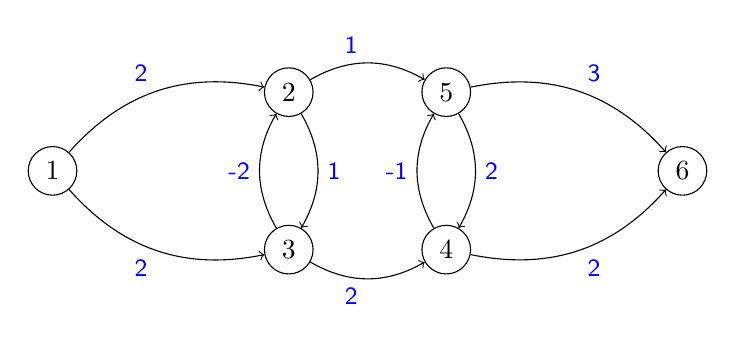
\begin{tikzpicture}
%\draw[->] (0,-2) -- (0,2) node [right] {$y$};  

%\foreach \i in {0,1,2,-1,-2}
%    \draw (-0.1, {\i}) -- (0.1, {\i}) node [left] {\i};
    
\node[circle,draw] (A1)  at (0,0) {1};
\node[circle,draw] (A2)  at (3,1) {2};
\node[circle,draw] (A3)  at (3,-1) {3};
\node[circle,draw] (A4)  at (5,-1) {4};
\node[circle,draw] (A5)  at (5,1) {5};
\node[circle,draw] (A6)  at (8,0) {6};

\path[every node/.style={font=\sffamily\small}]
    (A1) edge[->, bend left] node [blue, pos=0.5, above left] {2} (A2)
    (A1) edge[->, bend right] node [blue, pos=0.5, below left] {2} (A3)
    (A2) edge[->, bend left] node [blue, pos=0.5, right] {1} (A3)
    (A3) edge[->, bend left] node [blue, pos=0.5, left] {-2} (A2)
    (A2) edge[->, bend left] node [blue, pos=0.5, above left] {1} (A5)
    (A3) edge[->, bend right] node [blue, pos=0.5, below left] {2} (A4)
    (A4) edge[->, bend left] node [blue, pos=0.5, left] {-1} (A5)
    (A5) edge[->, bend left] node [blue, pos=0.5, right] {2} (A4)
    (A5) edge[->, bend left] node [blue, pos=0.5, above right] {3} (A6)
    (A4) edge[->, bend right] node [blue, pos=0.5, below right] {2} (A6);
\end{tikzpicture}
    
    Find the minimum cost route in (at most)
    \begin{enumerate}[label = {\textbf{(\greek*)}}]
        \item $L = 4$ steps
        
        \begin{sol}
        
        We define our objective function 
        
        $f_i(k) :=$ the length of the shortest path from \tc{1} to \tc{k} with at most $i$ arcs (steps)
    
    $1\leq k\leq 6,\quad 0\leq i\leq 4$
    
    Target: $f_4(6)$
    
    Boundary: $f_0(k)=
    \begin{cases} 
    0, & k=1 \\ \infty, & k\neq 1 
    \end{cases}$
    
    in fact, $f_i(1)=0$ for all $i\geq0$
    
    Our recursive formula for $2\leq k\leq 6,\quad 1\leq i\leq 4$ is 
    $$f_i(k) = \min\limits_{j\neq k} \{ f_{i-1}(j)+\alpha_{jk}\}$$
    
    \begin{itemize}
        \item[\underline{$i=1$}] \hspace{0.1cm} \\
    $\begin{aligned}
    f_1(2)&=2 & d(2)=1 \\
    f_1(3)&=2 & d(3)=1 \\
    f_1(k)&=\infty & k=4,5,6
    \end{aligned}$
    
    \item[\underline{$i=2$}] \hspace{0.1cm} \\
    $\begin{aligned}
    f_2(2)&=\min\cbr{f_1(1)+\alpha_{12},f_1(3)+\alpha_{32}} \\
    &=\min\cbr{0+2,2+(-2)}=0 & d(2)=3 \\
    f_2(3)&=\min\cbr{f_1(1)+\alpha_{13},f_1(2)+\alpha_{23}} \\
    &=\min\cbr{0+2,2+1}=2 & d(3)=1 \\
    f_2(4)&=f_1(3)+\alpha_{34} \\
    &= 2+2=4 & d(4)=3 \\
    f_2(5)&=f_1(2)+\alpha_{25} \\
    &= 2+1=3 & d(5)=2 \\
    f_2(6)&=\infty 
    \end{aligned}$
    
    \item[\underline{$i=3$}] \hspace{0.1cm} \\
    $\begin{aligned}
    f_3(2)&=\min\cbr{f_2(1)+\alpha_{12},f_2(3)+\alpha_{32}} \\
    &=\min\cbr{0+2,2+(-2)}=0 & d(2)=3 \\
    f_3(3)&=\min\cbr{f_2(1)+\alpha_{13},f_2(2)+\alpha_{23}} \\
    &=\min\cbr{0+2,0+1}=1 & d(3)=1 \\
    f_3(4)&=\min\cbr{f_2(3)+\alpha_{34},f_2(5)+\alpha_{54}} \\
    &=\min\cbr{2+2,3+2}=4 & d(4)=3 \\
    f_3(5)&=\min\cbr{f_2(2)+\alpha_{25},f_2(4)+\alpha_{45}} \\
    &=\min\cbr{0+1,4+2}=1 & d(5)=2 \\
    f_3(6)&=\min\cbr{f_2(4)+\alpha_{46},f_2(5)+\alpha_{56}} \\
    &=\min\cbr{4+2,3+3}=6 & d(6)=4 \ \text{or} \ 5
    \end{aligned}$
    
    \item[\underline{$i=4$}] \hspace{0.1cm} \\
    
    Our goal is $f_4(6)$ so we only need to evaluate that at this step:
    
    $\begin{aligned}
    f_4(6)&=\min\cbr{f_3(4)+\alpha_{46},f_3(5)+\alpha_{56}} \\
    &=\min\cbr{4+2,1+3}=4 & d(6)=5
    \end{aligned}$
    
    So our optimal route is
    
    $\tc{1}\to\tc{3}\to\tc{2}\to\tc{5}\to\tc{6}$
    
    with minimal cost $4$.
    \end{itemize}
    
    \end{sol}
        \item $L = 3$ steps
        
    \begin{sol}
        
        We already found $f_3(6)$ in the previous part of the question, i.e. $f_3(6)=6$ with decision(s) $d(6)=4$ or $5$
        
        And so our total cost is $6$, and our minimal routes are
        
        $\tc{1}\to\tc{2}\to\tc{5}\to\tc{6}$ \quad or \quad
        $\tc{1}\to\tc{3}\to\tc{4}\to\tc{6}.$
        \end{sol}
    \end{enumerate}
\end{prob}

\pagebreak
\begin{prob} %Problem 5 
    We need a specific equipment for $T = 4$ years. Each year we may take one of the following decisions:
    \begin{enumerate}[label = {(\roman*)}]
        \item to keep our equipment
        \item to replace our equipment with a new one
        \item to buy new equipment and sell our old one
    \end{enumerate}


The following costs may apply:

$\begin{aligned}
    k(t) 
    &= 1 + 2t 
    = \text{ the cost of using for one year period a machine of $t$ years old.} \\
    r(t, \tau ) 
    &= 3 + \tau + t 
    = \text{ the price for changing our $t$ years old equipment by a new one at the time $\tau$.} \\
    B(\tau ) 
    &= 5 + \tau 
    = \text{ the price of buying a new equipment at the time $\tau$.} \\
    s(t, \tau ) 
    &= 1 - t + \tau 
    = \text{ the profit of selling our $t$ years old equipment at the time $\tau$.}
\end{aligned}$


\begin{enumerate}[label = {\textbf{(\greek*)}}]
    \item Find the optimal policy (keep-replace-buy every year), provided that we start having an equipment of $t = 2$ years old.
    
    \begin{sol}
    
    \begin{enumerate}[start = 1, label = {\protect\tsc{$\mathbf{S_{\arabic*}}$}}]
    \item 
\begin{tikzpicture}
\foreach \i in {0,4}
\draw ({\i},-0.1) -- ({\i},0.1);
\node (T0) at (0,0) [below] {$\tau=0$};
\node (T1) at (4,0) [below] {$\tau=4$};
\draw (0,0) -- (4,0);
\end{tikzpicture}

$f(t,\tau):=$ the minimum cost for using the car of age $t$ from \tc{$\tau$} to \tc{$T$}.

Actions and costs (PO)):
\begin{itemize}
    \item \textbf{Keep}    \\ $k(t)+f(t+ 1,\tau+ 1)$
    \item \textbf{Replace} \\ $r(t)+k(0)+f(1,\tau+1)$
    \item \textbf{Buy} \\ $B(\tau)+k(0)-s(t,\tau)+f(1,\tau+1)$
\end{itemize}

Our objective function to optimize is, for $1\leq\tau<4$ and $t\geq1$

$\begin{aligned}
f(t,\tau) &=\min\cbr{ 1+2t+f(t+1,\tau+1),
                     3+\tau+t+1+f(1,\tau+1),
                     5+\tau+1-(1-t+\tau)+f(1,\tau+1)} \\
&= \min\begin{cases} 
1+2t+f(t+1,\tau+1), \\
4+\tau+t+f(1,\tau+1), \\
5+t+f(1,\tau+1)
\end{cases}
\end{aligned}$

Want to find $f(2,0)$ (we start with 2 year old equipment)

We have boundary condition: $f(t,T) =-s(t,T)=t-T-1=t-5$

\begin{tikzpicture}[scale=1.4]
\tikzset{
post/.style={->,shorten >=1pt,>=stealth',semithick}
}
\node (Tt) at (0,0) {$(t,\tau)$};
\node (T1) at (2,0) {$(1,\tau+1)$};
\node (Tt1) at (2,2) {$(t+1,\tau+1)$};
\node (Tt2) at (2,-2) {$(1,\tau+1)$};
\node[shape=circle,draw] (T3) at (5,0) {$T$};
\draw[post,rounded corners=5pt] (Tt) |- (Tt1) node [blue, pos=0.7, above] {$k(t)$} node [pos = 0.7, below] {Keep};
\draw[post,rounded corners=5pt] (Tt) |- (Tt2) node [blue, pos=0.7, below=1.5pt] {$\rbr{B(\tau)-s(t,\tau)}+k(0)$} node [pos = 0.7, above] {Buy};
%\draw[->] (Tt) -- (T1);
%\draw[->] (T1) -- (T3);
%\draw[->] (Tt1) -- (T3);
%\draw[->] (Tt2) -- (T3);

\path[every node/.style={font=\sffamily\small}]
    (Tt) edge[->] node [blue, pos=0.45, above] {$r(t,\tau)+k(0)$} node [pos=0.5, below] {replace}  (T1)
    (T1) edge[->] node [blue, pos=0.5, sloped, below] {$f(1,\tau+1)$} (T3)
    (Tt1.east) edge[->] node [blue, pos=0.5, sloped, above] {$f(t+1,\tau+1)$} (T3)
    (Tt2.east) edge[->] node [blue, pos=0.5, sloped, below] {$f(1,\tau+1)$} (T3);
\end{tikzpicture}

\item $\underline{\tau=4} \quad f(1,4)=-4, \ f(2,4)=-3,\dots,f(6,4)=1$

\item $\underline{\tau=3}$ Since we start with a 2 y.o. piece of equipment, either we've kept the equipment the whole time, so $t=2+3=5$, or we bought/replaced it at some point, so $1\leq t\leq 5$

$\begin{aligned}
f(1,3) &= \min\cbr{k(1)+f(2,4),r(1,3)+k(0)+f(1,4),\rbr{B(3)-s(1,3)}+k(0)+f(1,4)}\\
&= \min\cbr{3-3,7+1-4,8-3+1-4}=0 &\text{keep} \\
f(2,3) &= \min\cbr{k(2)+f(3,4),r(2,3)+k(0)+f(1,4),\rbr{B(3)-s(2,3)}+k(0)+f(1,4)}\\
&= \min\cbr{5-2,8+1-4,8-2+1-4}=3 &\text{keep or buy} \\
f(3,3) &= \min\cbr{k(3)+f(4,4),r(3,3)+k(0)+f(1,4),\rbr{B(3)-s(3,3)}+k(0)+f(1,4)}\\
&= \min\cbr{7-1,9+1-4,8-1+1-4}=4 &\text{buy} \\
f(4,3) &= \min\cbr{k(4)+f(5,4),r(4,3)+k(0)+f(1,4),\rbr{B(3)-s(4,3)}+k(0)+f(1,4)}\\
&= \min\cbr{9+0,10+1-4,8+0+1-4}=5 &\text{buy} \\
f(5,3) &= \min\cbr{k(5)+f(6,4),r(5,3)+k(0)+f(1,4),\rbr{B(3)-s(5,3)}+k(0)+f(1,4)}\\
&= \min\cbr{11+1,11+1-4,8+1+1-4}=6 &\text{buy} 
\end{aligned}$

$\underline{\tau=2}$ by the same argument as above, $1\leq t\leq 4$ 

$\begin{aligned}
f(1,2) &= \min\cbr{k(1)+f(2,3),r(1,2)+k(0)+f(1,3),\rbr{B(2)-s(1,2)}+k(0)+f(1,3)}\\
&= \min\cbr{3+3,6+1+0,7-2+1+0}=6 &\text{keep or buy} \\
f(2,2) &= \min\cbr{k(2)+f(3,3),r(2,2)+k(0)+f(1,3),\rbr{B(2)-s(2,2)}+k(0)+f(1,3)}\\
&= \min\cbr{5+4,7+1+0,7-1+1+0}=7 &\text{buy} \\
f(3,2) &= \min\cbr{k(3)+f(4,3),r(3,2)+k(0)+f(1,3),\rbr{B(2)-s(3,2)}+k(0)+f(1,3)}\\
&= \min\cbr{7+5,8+1+0,7+0+1+0}=8 &\text{buy} \\
f(4,2) &= \min\cbr{k(4)+f(5,3),r(4,2)+k(0)+f(1,3),\rbr{B(2)-s(4,2)}+k(0)+f(1,3)}\\
&= \min\cbr{9+6,9+1+0,7+1+1+0}=9 &\text{buy} 
\end{aligned}$

$\underline{\tau=1},\quad 1\leq t\leq 3$ 

$\begin{aligned}
f(1,1) &= \min\cbr{k(1)+f(2,2),r(1,1)+k(0)+f(1,2),\rbr{B(1)-s(1,1)}+k(0)+f(1,2)}\\
&= \min\cbr{3+7,5+1+6,6-1+1+6}=10 &\text{keep} \\
f(2,1) &= \min\cbr{k(2)+f(3,2),r(2,1)+k(0)+f(1,2),\rbr{B(1)-s(2,1)}+k(0)+f(1,2)}\\
&= \min\cbr{5+8,6+1+6,6+0+1+6}=13 &\text{any choice} \\
f(3,1) &= \min\cbr{k(3)+f(4,2),r(3,1)+k(0)+f(1,2),\rbr{B(1)-s(3,1)}+k(0)+f(1,2)}\\
&= \min\cbr{7+9,7+1+6,6+1+1+6}=14 &\text{replace or buy} 
\end{aligned}$

$\underline{\tau=0}$ goal at $t=2$ year old equipment we start with

$\begin{aligned}
f(2,0) &= \min\cbr{k(2)+f(3,1),r(2,0)+k(0)+f(1,1),\rbr{B(1)-s(2,0)}+k(0)+f(1,1)}\\
&= \min\cbr{5+14,5+1+10,5+1+1+10}=16 &\text{replace}
\end{aligned}$

\item Decision: Policy
\begin{enumerate}[start = 0, label = {$\tau=\arabic*:$}]
    \item replace\quad $\to (1,1)$
    \item keep\quad $\to (2,2)$
    \item buy\quad $\to (1,3)$
    \item keep\quad sell next year
\end{enumerate}

\end{enumerate}
    \end{sol}
    \item Prove that the strategy above remains the same, given that we start having an equipment of $t \geq 1$ years old.
    
    \begin{sol}
    
    We again have the objective function for $1\leq\tau<4$
    
    $f(t,\tau) = \min\begin{cases} 
1+2t+f(t+1,\tau+1), \\
4+\tau+t+f(1,\tau+1), \\
5+t+f(1,\tau+1)
\end{cases}$

With the same boundary condition $f(t,4)=t-5$

We wish to find $f(t,0)$ for arbitrary $t\geq 1$.

\begin{enumerate}
 
\item $\underline{\tau=3}$ 

$\begin{aligned}
f(t,3) &= \min\cbr{k(t)+f(t+1,4),r(t,3)+k(0)+f(1,4),\rbr{B(3)-s(t,3)}+k(0)+f(1,4)}\\
&= \min\cbr{1+2t+f(t+1,4),7+t+f(1,4),5+t+f(1,4)} \\
&= \min\cbr{1+2t+t+1-5,7+t+1-5,5+t+1-5}\\
&= \min\cbr{3t-3,t+3,t+1}\\
&=\begin{cases}
0, & t=1 \quad \text{keep}\\
3. & t=2 \quad \text{keep or buy}\\
t+1 & t\geq3 \quad \text{buy}
\end{cases}
\end{aligned}$

\item $\underline{\tau=2}$ 

$\begin{aligned}
f(t,2) &= \min\cbr{k(t)+f(t+1,3),r(t,2)+k(0)+f(1,3),\rbr{B(2)-s(t,2)}+k(0)+f(1,3)}\\
&= \min\cbr{1+2t+f(t+1,3),6+t+0,5+t+0} 
\end{aligned}$

But we know

$\begin{aligned}
f(t+1,3)&=\begin{cases}
3 & t=1 \\
t+2 & t\geq2 
\end{cases}
\end{aligned}$

And so

$\begin{aligned}
f(t,2) &= \min\cbr{1+2t+f(t+1,3),6+t,5+t} \\
&= \begin{cases}
\min\cbr{1+2+3,6+1,5+1}, & t=1\\
\min\cbr{1+2t+t+2,6+t,5+t}, & t\geq2\\
\end{cases}\\
&= \begin{cases}
\min\cbr{6,7,6}, & t=1\\
\min\cbr{3+3t,6+t,5+t}, & t\geq2\\
\end{cases}\\
&= \begin{cases}
6 & t=1 \quad \text{keep or buy}\\
t+5 & t\geq2 \quad \text{buy}
\end{cases}
\end{aligned}$

\item $\underline{\tau=1}$ 

$\begin{aligned}
f(t,1) &= \min\cbr{k(t)+f(t+1,2),r(t,1)+k(0)+f(1,2),\rbr{B(1)-s(t,1)}+k(0)+f(1,2)}\\
&= \min\cbr{1+2t+f(t+1,2),5+t+6,5+t+6} 
\end{aligned}$

But we know

$f(t+1,2)= t+6 \qquad t\geq1$

And so

$\begin{aligned}
f(t,1) &= \min\cbr{1+2t+t+6,11+t,11+t} \\
 &= \min\cbr{7+3t,11+t,11+t} \\
 &=\begin{cases}
 10 & t=1 \quad \text{keep}\\
 13 & t=2 \quad \text{any choice}\\
 11+t & t\geq3 \quad \text{replace or buy}
 \end{cases}
\end{aligned}$

$\underline{\tau=0}$ goal is $f(t,0)$

$\begin{aligned}
f(t,0) &= \min\cbr{k(t)+f(t+1,1),r(t,0)+k(0)+f(1,1),\rbr{B(0)-s(t,0)}+k(0)+f(1,1)}\\
&= \min\cbr{1+2t+f(t+1,1),4+t+10,5+t+10}\\
&= \min\cbr{1+2t+f(t+1,1),14+t,15+t}
\end{aligned}$

But we know

$\begin{aligned}
f(t+1,1) 
 &=\begin{cases}
 13 & t=1 \\
 12+t & t\geq2 
 \end{cases}
\end{aligned}$

And so 

$\begin{aligned}
f(t,0) &=\begin{cases}
\min\cbr{1+2t+13,14+t,15+t} & t=1\\
\min\cbr{1+2t+12+t,14+t,15+t} & t\geq2
\end{cases}\\
&=\begin{cases}
\min\cbr{14+2t,14+t,15+t} & t=1\\
\min\cbr{13+3t,14+t,15+t} & t\geq2
\end{cases}\\
&=14+t \qquad t\geq1 \qquad \text{replace}
\end{aligned}$

\item Decision: Policy
\begin{enumerate}[start = 0, label = {$\tau=\arabic*:$}]
    \item replace\quad $\to (1,1)$
    \item keep\quad $\to (2,2)$
    \item buy\quad $\to (1,3)$
    \item keep\quad sell next year
\end{enumerate}

Therefore we replace the car at year 1 regardless of its age $t\geq1$

And so the policy is the same for all $t\geq1$. Part $(\alpha)$ is just a particular case we validated above.
\end{enumerate}
    \end{sol}
\end{enumerate}

\end{prob}